\documentclass[titlepage]{article}
\usepackage[utf8]{inputenc}
\usepackage{geometry}[left = 1, right = 1, top = 1, bottom = 1] % 1 inch page margins
\usepackage[strict]{changepage} % adjust margins of certain sections within document
\usepackage{amsmath}
\usepackage{amssymb}
\usepackage{amsthm}
\usepackage{amsfonts}
\usepackage{textcomp}
\usepackage{graphicx} \graphicspath{{./}}
\usepackage{hyperref}

\setcounter{section}{-1}

% setup for amsthm package for writing proofs
\newtheorem{theorem}{Theorem}[section]
\renewcommand\qedsymbol{$\blacksquare$}
%\theoremstyle{definition}
\newtheorem{definition}{Definition}[section]
%\theoremstyle{lem}
\newtheorem{lem}{Lemma}[section]
\newtheorem{corollary}{Corollary}[section]

\title{\textbf{Project 1}\\\emph{Fast Trajectory Re-planning}}
\author{
    Zain Ali\\
    Michael Saunders\\
}
\date{Rutgers University\\Summer 2020}

\begin{document}
\maketitle
%\newpage

\section{Setup} Creating of grid worlds was completed by an algorithm which, when given x and y bounds, would create a .txt file with a grid of 1s and 0s. Prior to randomization, the algorithm first finds a random starting point and a random ending point and marks them as unblocked. It then runs through the entire matrix and assigns a node blocked at 30\% chance and unblocked at 70\%. 50 maps at size 101x101 are generated using this method.

\section{Understanding the Methods}
    
    \begin{figure}[h]
        \centering
        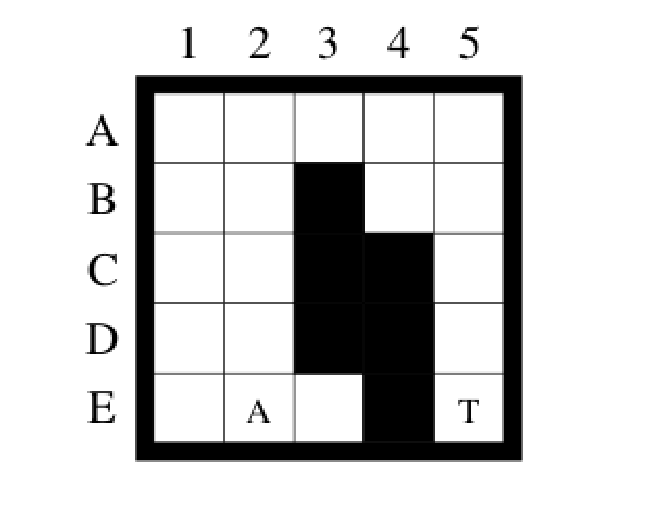
\includegraphics[scale = 0.5, trim = 0mm 10mm 0mm 0mm ]{figure8} %trim = <left> <bottom> <right> <top>
        \caption{A \textleftarrow{} agent, T \textleftarrow{} target}
        \label{fig:2ndexample}
    \end{figure}
    
    \noindent \textbf{a)} Consider the search problem in Figure \ref{fig:2ndexample}. It is an informed search in a finite space, in which each move costs 1. The agent knows where it is and it knows where the target is, but it does not know initially which cells are blocked. The agent can perceive the blocked-status of its direct neighbors, but no further. In the agent's initial state (E,2) it can see no blocked cells to the North, West, or East, and it knows it's up against a wall to the South. The agent also knows where the target lies (E,5). The cost-to-come for the agent's Northern neighbor (D,2) is 4, and its Eastern neighbor (E,3) is 2. The agent wants to reach the target effectively, so it chooses to move to the neighbor with the lowest cost-to-come (E,3). Only after moving will it learn the current path to the target is blocked. \\
    \\
    \noindent \textbf{b)} This project argues, in a finite grid-world, the agent is guaranteed to reach the target if it is not separated from it by blocked cells. Furthermore, if there is no path of unblocked cells from the agent to the target (thereby making it impossible for the agent to ever reach the target), the agent will stop searching and report this impossibility in finite time. \\
    \indent To show this is true, we need only to look at the mechanics of the A* search algorithm being used\footnote{The differences between Forward A*, Backward A*, and Repeated A* are irrelevant in the discussion on completeness}. A* tracks the visited cells in a list, and tracks the cells-to-be-visited (neighbors of the current cell) in a priority queue; cells are prioritized by increasing f-value.\footnote{A \emph{visited} cell will be considered "dead". The agent has been there, expanded all its neighbors, and determined it is not a viable path to the target. A \emph{blocked} cell is not a viable path to the target. So, if a cell is blocked, consider it visited.} \\
    \indent The agent will pop the highest-priority neighbor-cell out of the queue, and visit it. It will check to see if that cell is the target; if it is, the agent returns "target found". Otherwise the agent will look at the neighbors of the currently occupied cell, repeating the same process as before. Eventually the agent will find the target, or the priority queue of cells-to-be-visited will be empty and the agent will return informing us that a viable path to the target does not exist. Since the agent and the target exist in a finite grid-world, the process of searching for the target via the A* algorithm will be completed in finite time. Next, we will prove Theorem \ref{thm1}.
    
    \begin{adjustwidth}{20pt}{20pt}
        \begin{theorem}\label{thm1}
            \emph{The total number of moves of the agent $m$ until it reaches the target or discovers this is impossible, is bounded from above by the number of unblocked cells $u$ squared.}
            \[m <= u^2\]
        \end{theorem}
        
        \begin{proof}
            I don't see how the total number of moves of the agent could ever get close to the number of unblocked cells squared. \\
            Please give us Cheese for this part...
        \end{proof}
    \end{adjustwidth}
    
\section{The Effects of Ties}
In testing with both high-g and low-g tie breaking, high-g out preforms low-g in every case. In some cases, low-g tie breaking is significantly slower with the algorithm not being able able to arrive at the target in a realistic amount of time compared to high-g tie breaking. \\
\\
\noindent This can be explained with why high-g tie breaking is used in the first place. Given that the f-value is calculated using h(s) + g(s), it clear that if the f-value is need of a tie breaker, going with the high-g would mean the heuristic score is lower. Going with low-g would imply the heuristic is higher. This would be somewhat counter productive to the goal of the algorithm in attempting to arrive closer to the goal node with every move.

\break
\section{Forward vs. Backward A*}

    \begin{figure}[h!]
        \centering
        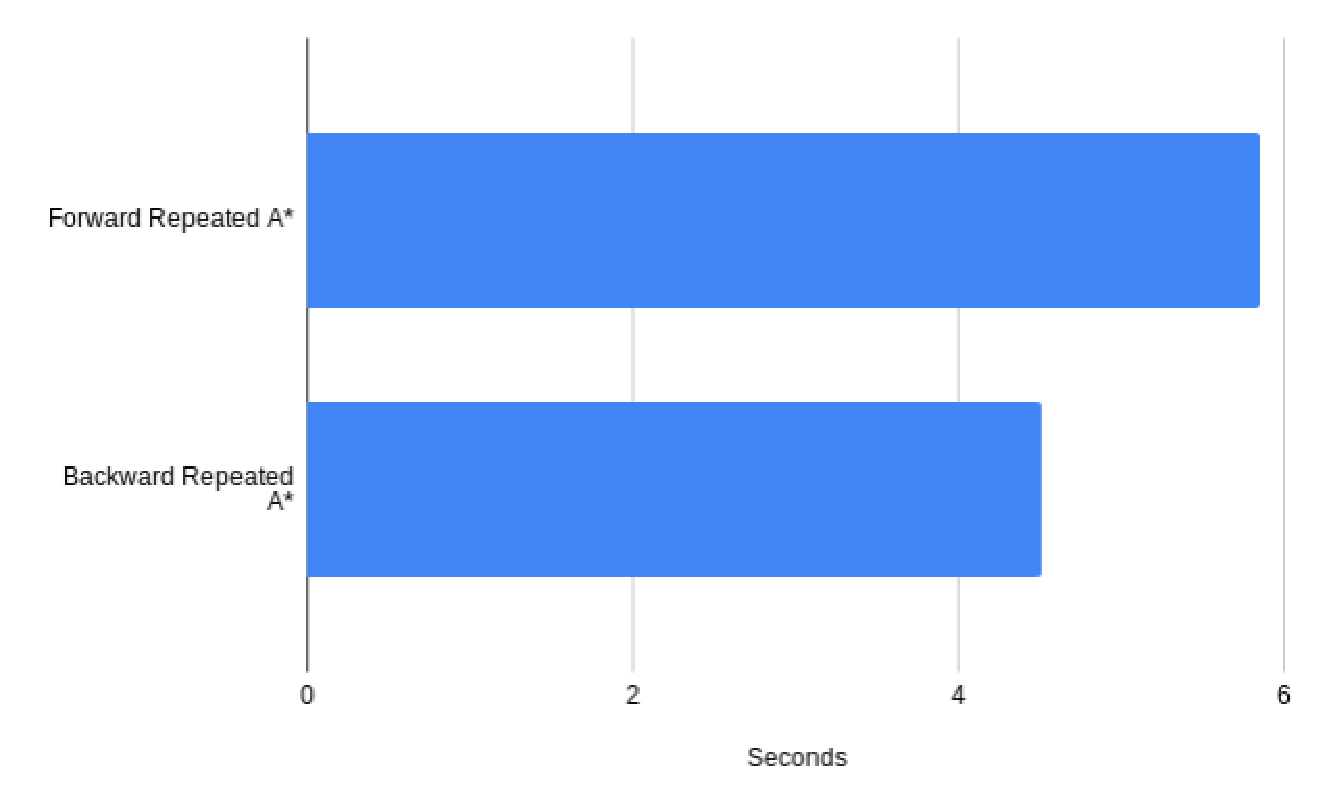
\includegraphics[scale = 0.5, trim = 20mm 10mm 0mm 0mm ]{AstarRuntime.eps} %trim = <left> <bottom> <right> <top>
        \caption{Run-time Comparison: Total time in seconds taken to search 50 grid worlds.}
        \label{fig:timecomp}
    \end{figure}
    
    \noindent Our implementation of Repeated Forward A* and Repeated Backward A* are essentially the same, but with the start states and goal states reversed. Both versions do break ties among cells with the same f-values by favoring the cell with the larger g-value.\\
    \indent Figure \ref{fig:timecomp}, represents the total time taken to run each version of Repeated A* on 50 different grid-worlds. As you can see, we found that Backward Repeated A* was faster in this case. We do believe it is likely that Forward Repeated A* could run faster in different grid-worlds. \\
    \indent If there happens to be a large chunk of blocked cells near the start state, then Forward A* may make extreme adjustments to avoid the large chunk, whereas Backward A* is not aware of the chunk until it gets much closer to its goal (the "start state"). There is a chance Backward A* can find a path through the large chunk to complete the search in less time. \\
    
%\break
\section{Heuristics in the Adaptive A*}

    \subsection{Consistency of Manhattan distances}
        \begin{figure}[h]
            \centering
            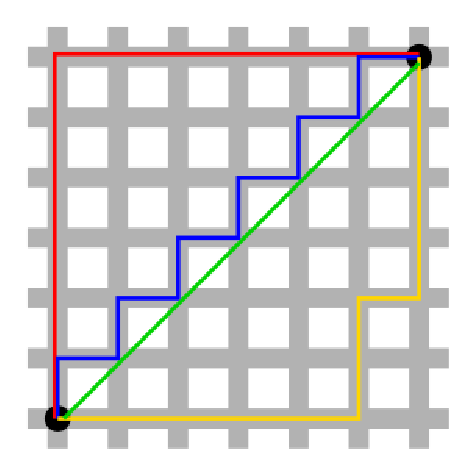
\includegraphics[scale = 0.7, trim = 0mm 0mm 0mm 0mm ]{Manhattan_distance.eps} %trim = <left> <bottom> <right> <top>
            \caption{Manhattan Distance Graphic.}\footnotemark
            \label{fig:taxicab}
        \end{figure}
        \footnotetext{\url{https://en.wikipedia.org/wiki/Taxicab_geometry}}
        %\noindent Figure \ref{fig:taxicab} is a representation of the Manhattan distance between two points on a two dimensional Cartesian plane.
        
    \begin{adjustwidth}{20pt}{20pt}
        
        \begin{theorem}\label{thm2}
            \emph{The Manhattan distances are consistent in grid-worlds in which the agent can move only in the four main compass directions.}\\
        \end{theorem} 
        
        \begin{definition}\label{manhattanD}
            \emph{The Manhattan distance \emph{d(p,q)} between two vectors \emph{p} and \emph{q} on a Cartesian plane is defined by equation \ref{manhattanD_eq}.}\\
            \begin{equation}\label{manhattanD_eq}
                d(p,q) = |p_x - q_x| + |p_y - q_y|
            \end{equation}\\
        \end{definition}
        
         \begin{lem}\label{trienql}
            \emph{The \textbf{triangle inequality} stipulates that each side of a triangle cannot be larger than the sum of the other two sides.\footnotemark}\\
             \footnotetext{Russel, Norvig; Artificial Intelligence, A Modern Approach; 3rd ed}
        \end{lem}
        
        \begin{definition}\label{consistency}
            \emph{A heuristic \emph{h(n)} is \textbf{consistent} if, for every node $n$ and every successor \emph{n'} of $n$ generated by any action $a$, the estimated  cost of reaching the goal from $n$ is no greater than the step cost of getting to \emph{n'} plus the estimated cost of reaching the goal from \emph{n'}.\footnotemark}
            \begin{equation}\label{const_eq}
                h(n) \leq c(n, a, n') + h(n')
            \end{equation}\\
            \footnotetext{Russel, Norvig; Artificial Intelligence, A Modern Approach; 3rd ed}
        \end{definition}
        
        \begin{corollary}\label{yahmon0}
            \emph{Let the target-state be notated as $G$. Consider $n$, $n'$, and $G$ to be three points on a triangle, and $c(x, y)$ to be the estimated Manhattan distance (i.e. cost) between any two states $x$ and $y$. Then \emph{c(n, G)}, \emph{c(n, n')}, and \emph{c(n', G)} correspond to the lengths of each side of that triangle.\\}
        \end{corollary}
        
        \begin{corollary}\label{yahmon1}
        \emph{Since \emph{h(x)} is the estimated cost from any state $x$ to $G$, we can deduce the following from Definition \ref{consistency} and Corollary \ref{yahmon0}:}
                \begin{equation*}
                    h(n) \xleftarrow{} c(n, G)
                \end{equation*}
                \begin{equation*}
                    c(n,a,n') \xleftarrow{} c(n, n')
                \end{equation*}
                \begin{equation*}
                    h(n') \xleftarrow{} c(n', G)
                \end{equation*}
        \end{corollary}
       
       \begin{proof}
            From the definition of Manhattan distances (Definition \ref{manhattanD}), triangle inequality (Lemma \ref{trienql}), and Corollary \ref{yahmon1}, it is clear Equation \eqref{const_eq} is true. The LHS of the inequality represents the length of one side of a triangle and the RHS represents the sum of the lengths of the other two sides of the same triangle. \\
            \\
            Theorem \ref{thm2} is true. Manhattan distances are consistent heuristics in grid-worlds in which the agent can move only in the four main directions.
       \end{proof}
       
       \begin{theorem}\label{thm3}
            \emph{Adaptive A* leaves initially consistent h-values consistent even if action costs can increase.}
       \end{theorem}
       
        \begin{proof}
           It is True that Cheese is tasty. Please give me cheese.
        \end{proof}
       
    \end{adjustwidth}
       
    
\section{Adaptive A* Run-time Comparison}
    \begin{figure}[h!]
        \centering
        \includegraphics[scale = 0.3, trim = 20mm 10mm 0mm 0mm ]{graph.eps} %trim = <left> <bottom> <right> <top>
        \caption{Run-time Comparison: Total average time in seconds taken to search 50 grid worlds.}
        \label{fig:timecomp}
    \end{figure}
    
    As seen in Figure 4, Adaptive A* \emph{can} be faster than Forward Repeated A*. However, this is not always the case. Even though Adaptive A* expands fewer nodes compared to Forward Repeated A*, when running on the same machine in succession, Forward Repeated A* is sometimes faster. On smaller grid words, the time it takes to run Adaptive A* or Repeated A* is on the order of thousands of a second. Small changes in the machine's speed can make small differences in the speed of the algorithm. Since they are not being run in parallel, small changes can add up to a noticeable in runtime over a period of 50 grid worlds. When run over the course of many attempts and grid world generations, the average runtime of Adaptive A* is seen to be slightly faster than Forward Repeated A*.
    
\section{Memory Issues}
For the architecture of this project, the grid world is stored in memory with each node in the grid having its own attributes. These attributes unfortunately take up a lot of memory. With that, there are two of these saved. One with the agent's view, and the other with the entire maze. When measuring using Python's built in object size calculator and adding up the values, the State object uses up 216 Bytes. With each node being a State. This would make the size of running on a 101x101 grid world be $216*(101*101) = 2,203,416 Bytes = 2.2MB$. Using the same calculation on a 1001x1001 grid world, we would get $216*(1001*1001) = 216,432,216 Bytes = 216.43 MB$.\\
\\
In order to find what size grid world can be run with 4 MB, we can use $216*N^2 = 4,000,000 Bytes$ where we solve for N. The variable N in this case a dimension in a NxN grid world. We would end up with being able to host a size 136x136 grid world. This is not much larger than the 101x101 grid world that we tested on, so there are definitely ways the size can be reduced. The main thing is that it would be helpful to have a separate smaller object for the unaltered grid world being saved in memory. Much of the state object is used only when dealing with what the agent has seen, so there is no need for the excess unused memory for the world matrix.

\section*{Final Thoughts}
A place to wrap it up if we want to.

\end{document}
